%!Tex root=ZF_bmicha_TRM.tex
\subsection{Denavit-Hartenberg (DH) Convention}
    \vspace{0.5em}
    \begin{center}
        \fbox{%
            \parbox{0.95\linewidth}{%
                The $x_i$ axis must be \textbf{perpendicular} and \textbf{intersect} the $z_{i-1}$ axis.
            }
        }
    \end{center}

    \begin{minipage}{0.54\linewidth}
        \begin{center}
            \resizebox{\linewidth}{!}{
                    \includegraphics[
                        page = {8},
                        trim = {16cm, 7cm, 7cm, 4cm}, %left bottom right top
                        clip
                    ]{Forward_Kinematics/03_2020-10-13_ForwardKinematics.pdf}
                }
        \end{center}
    \end{minipage}
    \begin{minipage}{0.45\linewidth}
        \small
        \begin{description}
            \item[\boldmath{$\theta$}:] \textbf{joint angle}\\ (about original z-axis) 
            \item[\boldmath{$d$}:]      \textbf{link offset}\\ (along original z-axis) 
            \item[\boldmath{$a$}:]      \textbf{link length}\\ (along current x-axis) 
            \item[\boldmath{$\alpha$}:] \textbf{link twist} \\ (about current x-axis) 
        \end{description}
    \end{minipage}
    \subsubsubsection{Example}
    \vspace{0.5em}
    \begin{minipage}{0.5\linewidth}
        \begin{center}
            \resizebox{\linewidth}{!}{
                    \includegraphics[
                        page = {9},
                        trim = {2.5cm, 1.5cm, 20.5cm, 4cm}, %left bottom right top
                        clip
                    ]{Forward_Kinematics/03_2020-10-13_ForwardKinematics.pdf}
                }
        \end{center}
    \end{minipage}
    \hfill
    \begin{minipage}{0.39\linewidth}
        \begin{center}
            \resizebox{\linewidth}{!}{
                    \includegraphics[
                        page = {9},
                        trim = {16.7cm, 6.3cm, 8.42cm, 8.7cm}, %left bottom right top
                        clip
                    ]{Forward_Kinematics/03_2020-10-13_ForwardKinematics.pdf}
                }
        \end{center}
    \end{minipage}
    
    
    
    \subsubsubsection{Homogeneous Transformation}
        \begin{center}
            All operations w.r.t. \textbf{current frame!}
        \end{center}
        $$\boxed{
            A_i = \textrm{Rot}_z(\theta)\ \textrm{Trans}_z(d)\ \textrm{Trans}_x(a)\ \textrm{Rot}_x(\alpha) = H_i^{i-1}
        }$$
        {\scriptsize
        $$
            =
            \begin{bmatrix}
                c_\theta & -s_\theta & 0 & 0\\
                s_\theta & c_\theta & 0 & 0\\
                0 & 0 & 1 & 0\\
                0 & 0 & 0 & 1\\
            \end{bmatrix}\!\!
            \begin{bmatrix}
                1 & 0 & 0 & 0\\
                0 & 1 & 0 & 0\\
                0 & 0 & 1 & d\\
                0 & 0 & 0 & 1\\
            \end{bmatrix}\!\!
            \begin{bmatrix}
                1 & 0 & 0 & a\\
                0 & 1 & 0 & 0\\
                0 & 0 & 1 & 0\\
                0 & 0 & 0 & 1\\
            \end{bmatrix}\!\!
            \begin{bmatrix}
                1 & 0 & 0 & 0\\
                0 & c_\alpha & -s_\alpha & 0\\
                0 & s_\alpha & c_\alpha & 0\\
                0 & 0 & 0 & 1\\
            \end{bmatrix}
        $$
        $$
            = 
            \begin{bmatrix}
                c_\theta & -s_\theta c_\alpha &  s_\theta s_\alpha & a c_\theta\\
                s_\theta &  c_\theta c_\alpha & -c_\theta c_\alpha & a s_\theta\\
                0        &  s_\alpha          &  c_\alpha          & d\\
                0        &  0                 &  0                 & 1
            \end{bmatrix}
        $$}
    \subsubsubsection{Choosing Axis}
            \begin{enumerate}
                \item Set z axis along rotational or translational axis
                \item Set x axis according to DH convention
                \item Set y axis using right hand rule
            \end{enumerate}
        
\subsection{Definitions}
    \subsubsection{Workspaces}
        \textbf{Reachable Workspace:} EE Origin can reach with at least 1 orientation\\
        \textbf{Dexterous Workspace:} EE Origin can reach with multiple orientations
    \subsubsection{Joint- \& Taskspace}
        \textbf{Jointspace:} Independent, actuated parameters\\
        \textbf{Taskspace:} Position \& orientation of EE
